%This is a LaTeX template for homework assignments
\documentclass{article}
\usepackage[utf8]{inputenc}
\usepackage{amsmath}
\usepackage{graphicx}
\usepackage{float}

\begin{document}

\section*{Taller 1 - Gravimetr\'ia}
Nombre: Carol Vanessa Barrera L\'opez 
\\ C\'odigo: 201514934
\\Fecha: Septiembre de 2017

\subsection*{1.1 Modelamiento de anomal\'ias gravim\'etricas para sistemas sencillos} 

\begin{enumerate}%starts the numbering

\item {\bf Esfera:} Modelo para los diapiros.
	\begin{enumerate}
	\item Demostraci\'on de la ecuaci\'on:
	El efecto de gravedad en un punto P de una esfera en direcci\'on $d$ (donde $d$ es la distancia del centro de la esfera al punto) es  $g_d =\frac{GM}{d^{2}}$. Pero debemos hallar la componente vertical, por lo tanto $g = g_d\cos(\theta)$. Como $\cos(\theta)= \frac{z}{d}$, obtenemos entonces que $g =\frac{GMz}{d^{3}}$ (1). La masa en este caso se expresa como la diferencia de densidades entre el suelo($\rho_s$) y la esfera($\rho_e$), y el volumen de la esfera, obteniendo as\'i que $M = (\rho_e-\rho_s)\frac{4}{3}r^{3}\pi $. Ahora expresamos $d$ en t\'erminos de $x$ (la distancia en superficie del punto P al centro de la esfera) y $z$ (profundidad de la esfera), $d = (x^{2}+z^{2})^{\frac{1}{2}}$. Reemplazamos en (1) todo lo anterior, obteniendo as\'i que
\begin{equation*}
g(x) = G(\rho_e-\rho_s)\frac{4}{3}r^{3}\pi \frac{z}{(x^{2}+z^{2})^{\frac{3}{2}}}
\end{equation*}

El $g_{max}$ se obtendr\'ia en $x=0$ (cuando estamos sobre la esfera) y ser\'ia 
\begin{equation*}
g_{max}(x) = G(\rho_e-\rho_s)\frac{4}{3}r^{3}\pi \frac{1}{z^{2}}
\end{equation*}

	\item Se realiz\'o una gr\'afica con tres curvas de la anomal\'ia para diferentes z, cuando la densidad de la esfera era mayor a la densidad del suelo y una curva mostrando la anomal\'ia consecuente a una esfera con una densidad menor que la densidad del suelo (caso del diapiro).Se puede observar que a mayor z, la curva de la anomal\'ia gravitacional tiene menor altura (por ende menor gmax). Esto se debe a que la relaci\'on entre $g(x)$ y $z$ es inversamente proporcional. Tambi\'en se puede observar que a mayor z, la curva es m\'as ancha, siendo menos clara la anomal\'ia. En el caso del diapiro se puede observar como obtenemos una anomal\'ia negativa. Esto se debe a que la relaci\'on entre $g(x)$ y $M$ es directamente proporcional, por ende si la densidad de la esfera es menor, la gravedad que va a ejercer con respecto al suelo va a ser menor de igual manera.
	\begin{figure}[H]\centering 
	\includegraphics[width=10cm]{AEsfera.pdf}
	\end{figure}
	\item Se calcularon los half-with, $x_{med}$ de todas las configuraciones para cuando $g = g_{max}/2$ . Luego se hall\'o el coeficiente entre $x_{med}$ y z. Se obtuvo valores de 1.32, 1.332, 1.331 y 1.32. En promedio todas las razones se pueden aproximar a 1.3, lo cual nos indica que la profundidad(z) y el $x_{med}$ del perfil est\'an relacionados de manera directamente proporcional por una constante, siendo $x_{med}$ 1.3 veces $z$.
	\end{enumerate}

\item {\bf Cilindro:} Modelo para anticlinales y sinclinales.
	\begin{enumerate}
	\item El valor m\'aximo de la gravedad ($g_{max}$) en el caso de un cilindro infinito de radio $r$, densidad $\rho_c$, enterrado horizontalmente a una profundidad z es: 
	\begin{equation*}
	g_{max} = 2\pi G(\rho_c-\rho_s)r^{2}\frac{1}{z}
	\end{equation*}
	\item Se realiz\'o una gr\'afica con tres curvas de anomal\'ia para diferentes z con una densidad del cilindro mayor a la densidad del suelo. Se observan las mismas tendencias que en el caso de la esfera. Se puede observar que a mayor z, la curva de la anomal\'ia gravitacional tiene menor altura (por ende menor gmax) y tambi\'en se puede observar que a mayor z, la curva es m\'as ancha, siendo menos clara la anomal\'ia. Esto se debe a que, como se dijo anteriormente, la relaci\'on entre $g(x)$ y $z$ es inversamente proporcional, por ende si aumentamos la profundidad, disminu\'imos la anomal\'ia gravim\'etrica.
	\begin{figure}[H]\centering
	\includegraphics[width=10cm]{ACilindro.pdf}
	\end{figure}
	\item Se calcularon los half-with como se hizo con los perfiles del modelo de la esfera. Luego se hall\'o el coeficiente entre $x_{med}$ y $z$. Se obtuvo valores de 0.99, 0.999 y 0.998. Esto quiere decir que z esta relacionada con elhalf-with del perfil de manera directamente proporcional en un factor 1:1.
	\end{enumerate}
\item {\bf Losa horizontal semi-infinita:} Modelo de una falla vertical.
	\begin{enumerate}
	\item El perfil de anomal\'ia gravitacional tomado perpendicularmente al l\'imite de una losa con grosor $h$, densidad $\rho_l$, enterrada a una profundidad $z$ es:
	\begin{equation*}
	g(x) = 2G(\rho_l-\rho_s)h[\frac{\pi}{2} + \arctan(\frac{x}{z})]
	\end{equation*}
	\item Se realiz\'o una gr\'afica con tres curvas de anomal\'ia para diferentes z, diferentes grosores y diferentes densidades. En ella se puede apreciar que la anomal\'ia es mayor si se aumenta el grosor y la densidad de la losa, variables relacionadas con la masa, la cual es directamente proporcional a $g(x)$. Como los modelos anteriores, si se aumenta la profundidad (z), la anomal\'ia va a disminuir y tambi\'en la claridad de donde se encuentra el objeto que la produce, es decir, el cambio no va a ser tan marcado, como se puede evidenciar con la losa m\'as somera y la m\'as profunda en el diagrama.(densidades en [kg/$m^{3}$]).
	\begin{figure}[H]\centering
	\includegraphics[width=10cm]{ALosa.pdf}
	\end{figure}
	\item Se realiz\'o una gr\'afica con la primera y la segunda derivada de los perfiles de anomal\'ias obtenidos anteriormente. Se puede ver como la primera derivada se asemeja a los perfiles de anomal\'ia de los modelos de la esfera y del cilindro. Esta tendencia se debe a que es en ese sector donde se presenta el cambio dr\'astico de la medida de gravedad. En cuanto a la segunda derivada se puede decir que se asemeja al perfil de anomal\'ia generado por una falla, en la cual la anomal\'ia positiva se asocia con la secci\'on de la placa que sube y la anomal\'ia negativa con aquel que baja.
	\begin{figure}[H]\centering
	\includegraphics[width=8cm]{derivadas.pdf}
	\end{figure}
	\end{enumerate}
\end{enumerate}%ends the numbering

\subsection*{1.2 M\'etodo de Nettleton, correcciones de Bouger y Aire libre}

\begin{enumerate}%starts the numbering
\item Con los datos del archivo del taller 1.2, hoja 1, se aplic\'o el m\'etodo de Nettleton para obtener la densidad de la roca principal. Primero se realiz\'o la gr\'afica de la topograf\'ia del perfil. Se obtuvieron las correcciones de Aire libre y de Bouger. Para el caso de la anomal\'ia de Bouger, se calcul\'o con distintos valores de densidad hasta que se obtuvo la densidad \'optima, que fue de 2750 kg/$m^{3}$.
\begin{figure}[H]\centering
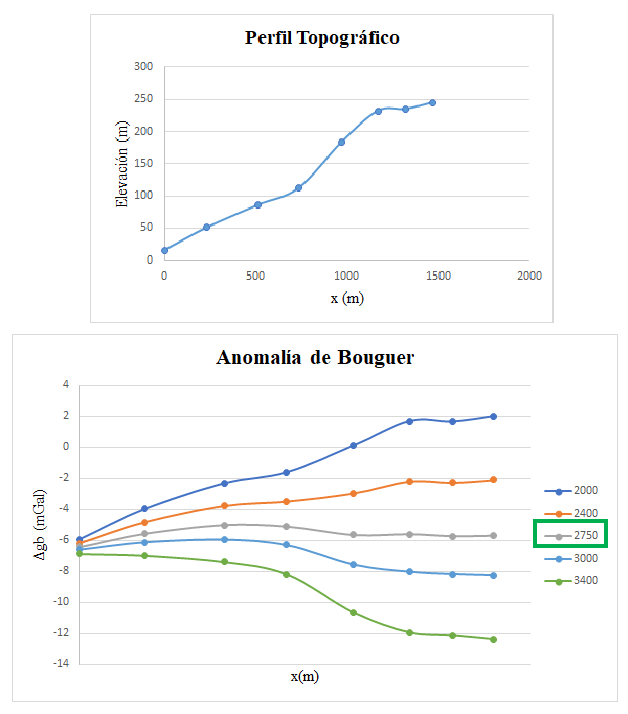
\includegraphics[width=10cm]{Densidad.png}
\end{figure}
\item Posteriormente (con los datos del mismo archivo pero de la hoja dos), se calcularon las anomalias de Aire Libre y Bouger para cada estaci\'on, usando la densidad \'optima calculada en el punto anterior. Se realiz\'o la anomal\'ia de Bouger en funci\'on de la distancia sobre el perfil:
\begin{figure}[H]\centering
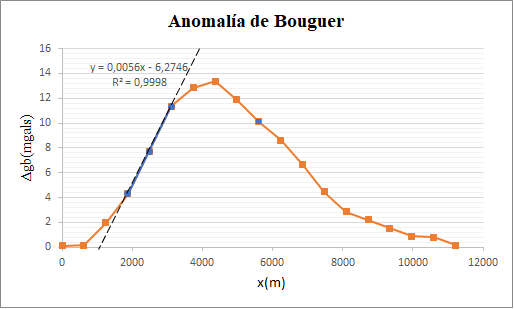
\includegraphics[width=10cm]{Volcan.png}
\end{figure}
\item La anomal\'ia de Bouguer muestra una anomal\'ia centrada en el volc\'an. Se hace un an\'alisis con el modelo de la esfera: 
	\begin{enumerate}
	\item Para ello se hall\'o el half-with ($x_{med}$) [Centrando la anomal\'ia en el $g_{max}$, y calculando los x con la linea de tendencia (en el caso del segundo x se ubica la linea de tendencia con pendiente negativa en el punto azul), como se muestra en la gr\'afica]. Hecho lo anterior, se procede a calcular el $x_{med}=$  3902.58 m.  Como se vi\'o en la secci\'on 1.1, la raz\'on entre $x_{med}$ y $g_{max}$ es una constante igual a 1.3, por lo tanto obtenemos que la profundidad a la que se encuentra la esfera es de $z =$ 3002 m aproximadamente. 
	\item Si se asume una diferencia de densidades ($(\rho_e-\rho_s)$) de 200 kg/$m^{3}$, y despejando en la ecuaci\'on $r$:
	\begin{equation*}
	r = (\frac{3}{4}\frac{(x^{2}+z^{2})^{\frac{3}{2}} g(x)}{G(\rho_e-\rho_s)\pi z})^{\frac{1}{3}}
	\end{equation*}
	obtenemos que $r=$ 2246 m aproximadamente.
	\item La presencia de esa esfera bajo un  volc\'an con actividad reciente puede deberse a la c\'amara magm\'atica, la cual al contener fundido de roca presenta una densidad mucho menor que la roca de caja (s\'olida) en la que se encuentra emplazada pero genera una elevaci\'on considerable del terreno. 
	\end{enumerate}
\end{enumerate}%ends the numbering

\subsection*{1.2 Visualizaci\'on de datos gravim\'etricos y an\'alisis}

\begin{enumerate}%starts the numbering
\item A partir de los datos topogr\'aficos y gravim\'etricos encontrados en el archivo del taller 1.3 se realiza un mapa de elevaci\'on del terreno con localizaci\'on de la estaci\'on base y las estaciones gravim\'etricas (a), un Mapa de contornos para la anomal\'ia de aire libre (b) y un Mapa de contornos para la anomal\'ia de Bouger(c):
	\begin{enumerate}
	\begin{figure}[H]\centering
	\item 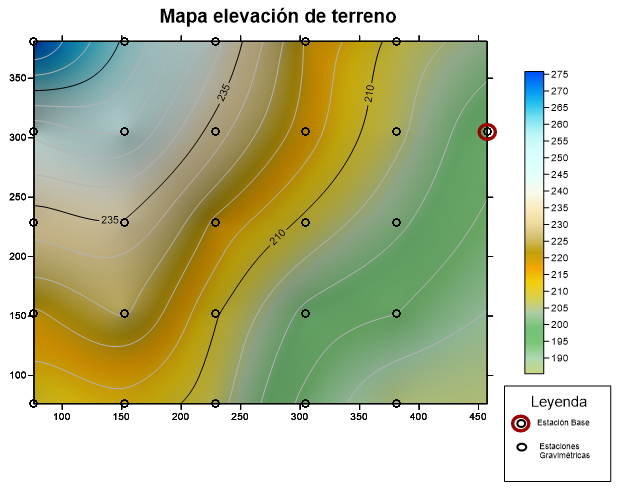
\includegraphics[width=8cm]{ElevacionTerreno.png}
	\end{figure}
	\begin{figure}[H]\centering
	\item 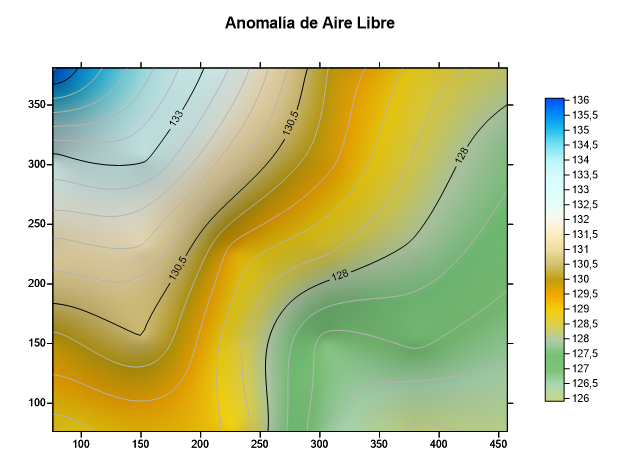
\includegraphics[width=8cm]{AAireLibre.png}
	\end{figure}
	\begin{figure}[H]\centering
	\item 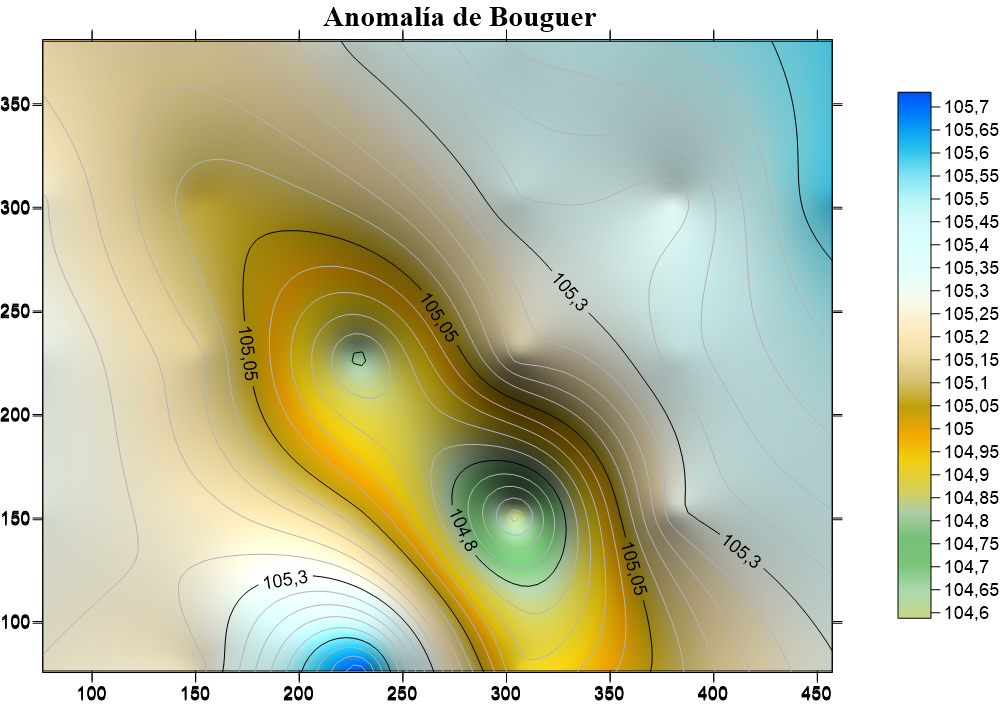
\includegraphics[width=8cm]{ABouguer.png}
	\end{figure}
	\end{enumerate}
En primer lugar se puede ver que el mapa de contornos de la anomal\'ia de Aire Libre se asemeja mucho al mapa de elevaci\'on de terreno debido a que esta anomal\'ia solo tiene en cuenta el cambio de la gravedad con respecto a la altura al elipsoide de referencia. Con respecto al mapa de contornos de la anomal\'ia de Bouger, podemos observar lo que dif\'icilmente se pod\'ia distinguir en el mapa de elevaci\'on de terreno. Como la anomal\'ia de Bouger quita la contribuci\'on del material entre la elipsoide de referencia y la estaci\'on, demarca muy bien los puntos en los cuales la estaci\'on se encuentra a una altura mucho m\'as elevada que el resto del terreno. Es as\'i como se ven claramente un par de picos en donde la correcci\'on fue mucho mayor (verde) y tambi\'en unas zonas donde la correcci\'on fue m\'inima (en azul).
\item A partir de los datos cartogr\'aficos y gravim\'etricos de Colombia gener\'e:
	\begin{enumerate}
	\item Un mapa de elevaci\'on del terreno de Colombia mostrando los l\'imites departamentales (en l\'ineas negras) y cuencas sedimentarias (en l\'ineas cafe claro).
	\begin{figure}[H]\centering
	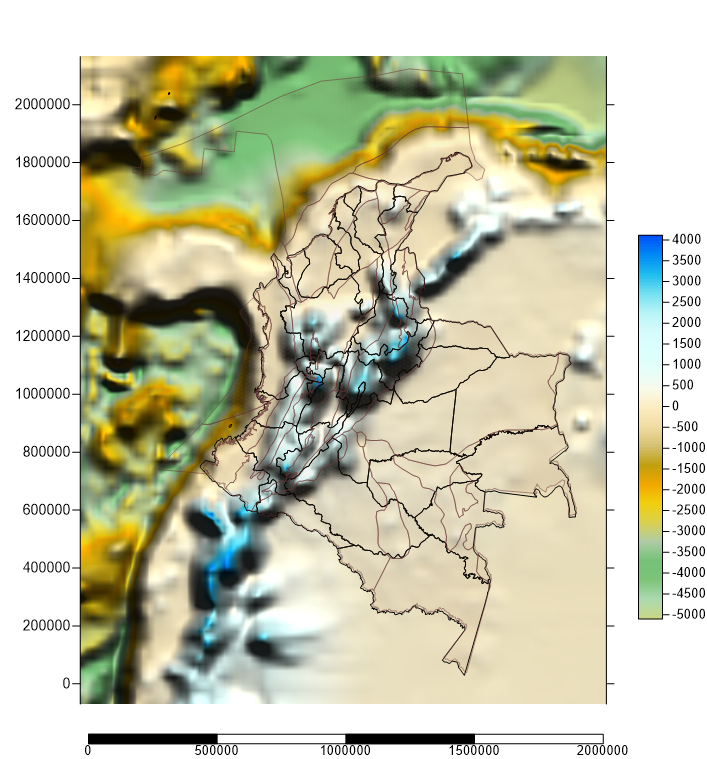
\includegraphics[width=8cm]{TColombia.png}
	\end{figure}
	\item Un mapa de Anomal\'ia de Bouger Total de Colombia (AHN, 2010), donde se puede ver que en la zona sobre la corteza oce\'anica la anomal\'ia es positiva y muy grande debido a que se encuentra por debajo de la elipsoide de referencia. Tambien se puede observar que es positiva en la zona m\'as alejada al borde continental, esto posiblemente a que es el crat\'on continental que es muy viejo y a pasado por mucho tiempo por el proceso de erosi\'on, lo cual llev\'o a crear cuencas sedimentarias y adem\'as lo dej\'o en equilibrio isost\'atico , contrario a los bordes convergentes, donde se est\'a elevando la corteza (por orogenia y el vulcan\'ismo generado por la fusi\'on parcial en la zona de subducci\'on) y por ende, la anomal\'ia de Bouger es negativa (Puesto que est\'a por encima de la elipsoide de referencia).
	\begin{figure}[H]\centering
	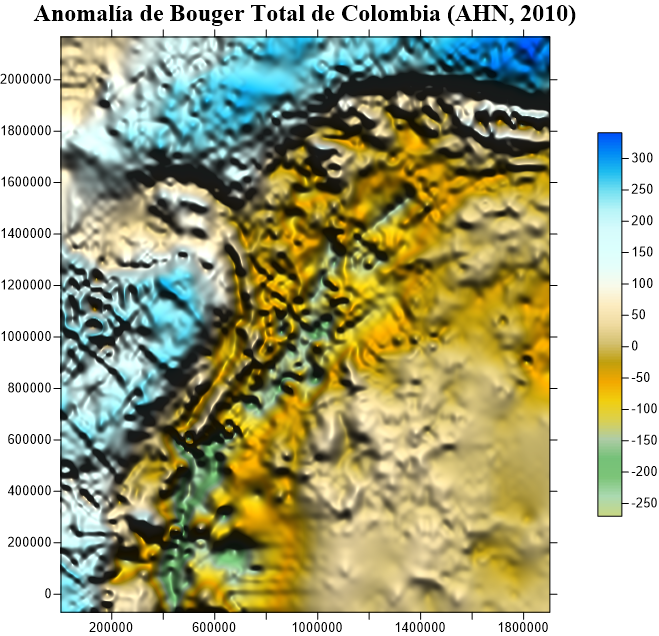
\includegraphics[width=10cm]{CBAColombia.png}
	\end{figure}
	\item Un mapa con el gradiente del mapa de Anomal\'ia de Bouger total de colombia y tambi\'en un mapa de la primera derivada en direcci\'on perpendicular a la tendencia de las fallas geol\'ogicas del pa\'is. Se puede observar como en el mapa del gradiente de la anomal\'ia de Bouger resaltan los cambios abruptos en la topograf\'ia de Colombia, como las cordilleras (Oriental, central y occidental), los arcos volc\'anicos y los l\'imites entre placas (que son los que m\'as resaltan. En el caso del mapa con la derivada en direcci\'on perpendicular a la tendencia de las fallas geol\'ogicas del pa\'is, se puede ver como estas mismas se ven con mucha m\'as claridad. Se correlaciona este con los datos suministrados de las fallas y se ve como las anomal\'ias se presentan en la m\'isma ubicaci\'on geogr\'afica que los datos de las fallas del pa\'is.
	\begin{figure}[H]\centering
	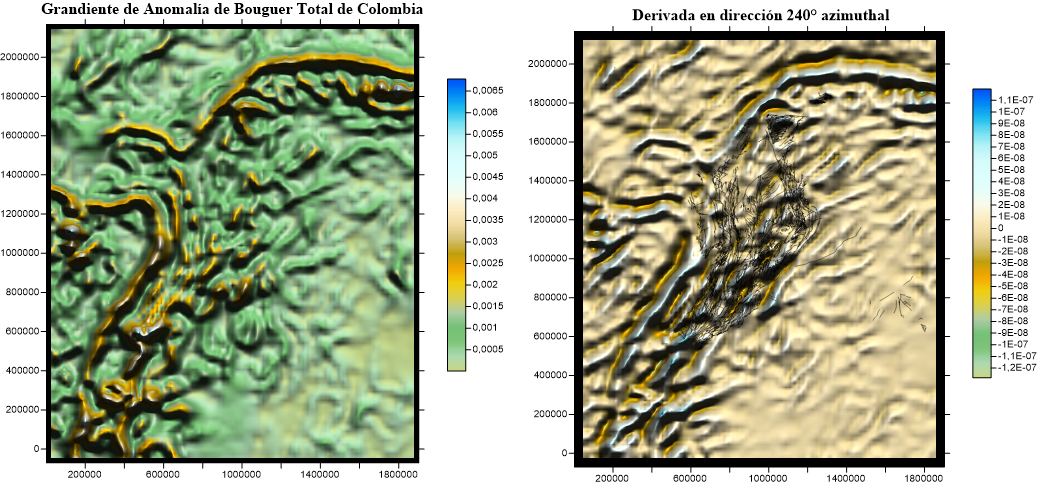
\includegraphics[width=12cm]{DerivadasCBACol.png}
	\end{figure}
	\end{enumerate}

\end{enumerate}%ends the numbering

\end{document}







